\documentclass[12pt,ngerman,parskip=half]{scrartcl}

\usepackage{babel}
\usepackage{blindtext}
\usepackage{tikz}

\usepackage{tikz}
\usetikzlibrary{automata, positioning, arrows}

\begin{document}

\section{Basics}

\blindtext

\begin{center}
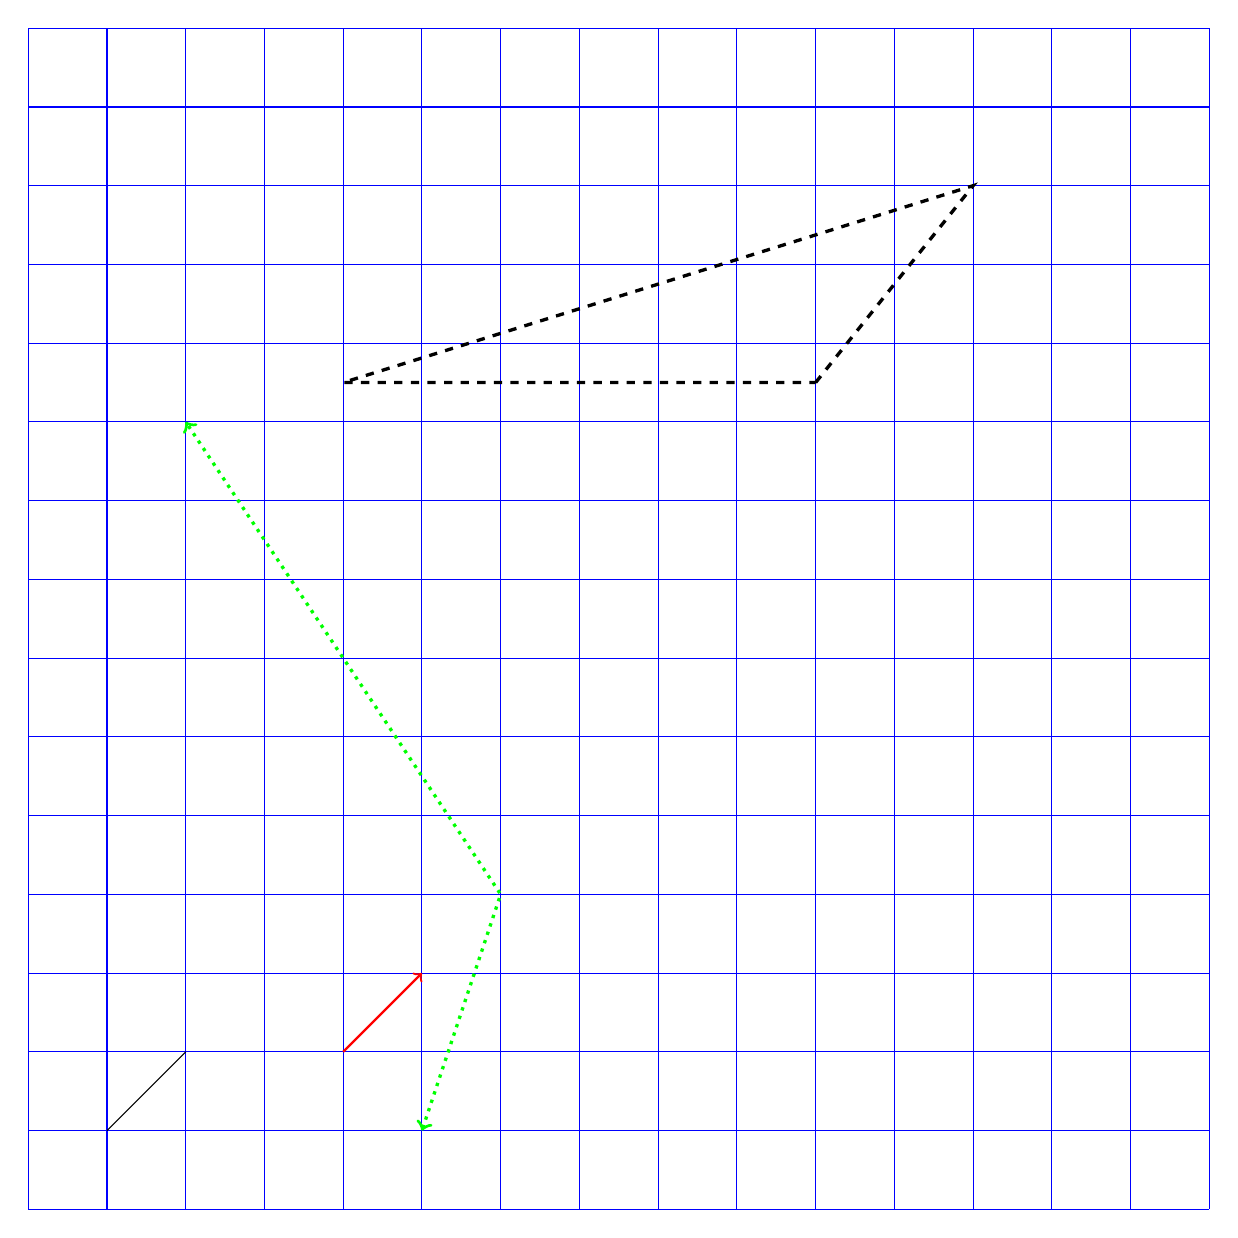
\begin{tikzpicture}
\draw[help lines,blue,thin] (0,0) grid (15,15);
\draw (1,1) -- (2,2);

\draw[->,thick, red] (4,2) -- (5,3);

\draw[<->, very thick, green, dotted] (5,1) -- (6,4) -- (2,10);

\draw[very thick, black, dashed] (10,10.5) -- (12,13) -- (4,10.5) -- cycle;

\end{tikzpicture}
\end{center}

\blindtext

\section{Relative und Polar-Koordinaten}

\begin{center}
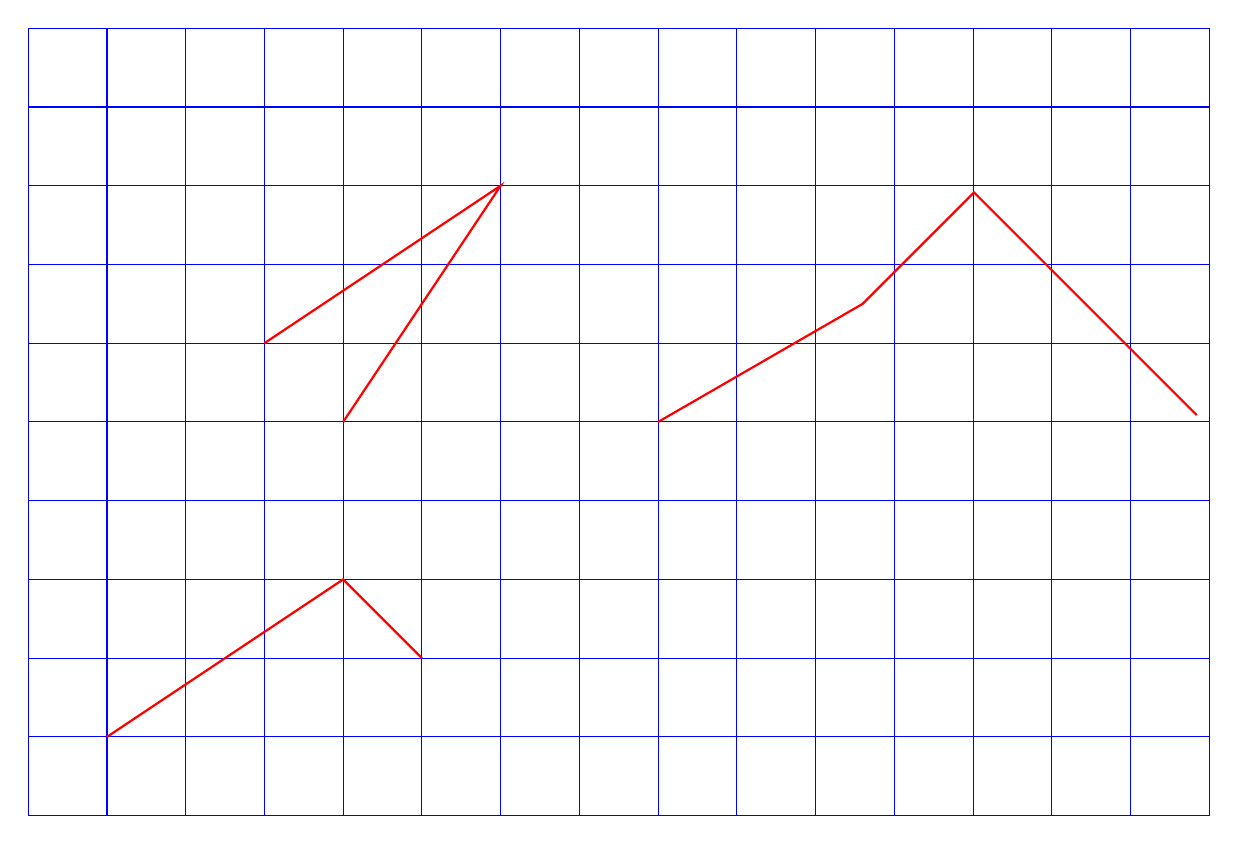
\begin{tikzpicture}
\draw[help lines,blue,thin] (0,0) grid (15,10);

% Relative Koordinaten mit Wechsel des Ursprungs
\draw[thick, red](1,1) -- ++(3,2) -- ++(1,-1);

% Relative Koordinaten ohne Wechsel des Ursprungs
\draw[thick, red](3,6) -- +(3,2) -- +(1,-1);

% Polarkoordinaten
\draw[red,thick](8,5) -- ++(30:3) -- ++(45:2) -- ++(-45:4);
\end{tikzpicture}
\end{center}

\section{Knoten = Nodes}

\begin{center}
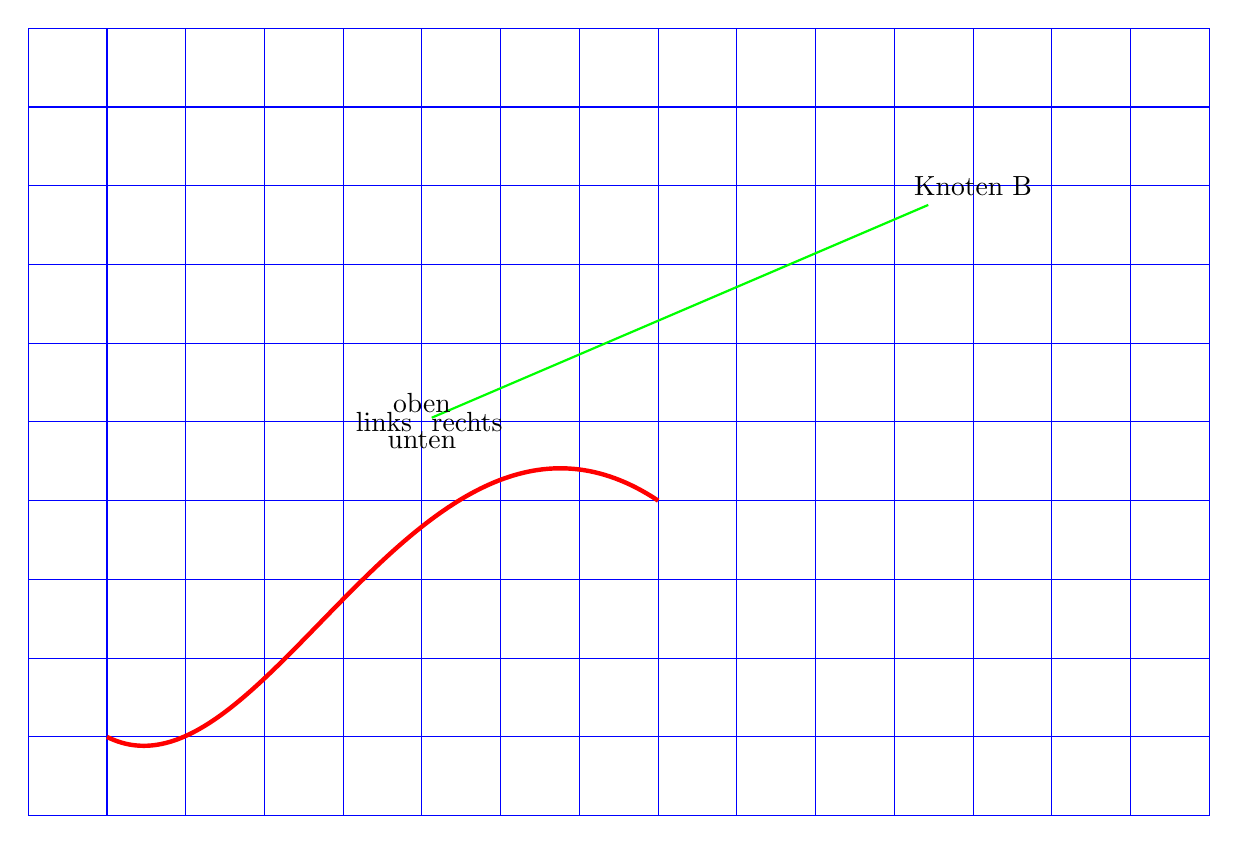
\begin{tikzpicture}
\draw[help lines,blue,thin] (0,0) grid (15,10);

\node [] (A) at (5,5){};

\node (B) at (12,8){Knoten B};
\draw[thick, green] (A) -- (B);

\node[below] at (A) {unten};
\node[above] at (A) {oben};
\node[left] at (A) {links};
\node[right] at (A) {rechts};

\draw[ultra thick, red](1,1) .. controls (3,0) and (5,6) .. (8,4);

\end{tikzpicture}
\end{center}

\blindtext

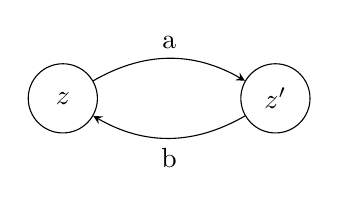
\begin{tikzpicture}[node distance=2.7cm]
\node[state] (z) {$z$};
\node[state, right of=z] (z2) {$z'$};
\draw [-stealth]
(z) edge[bend left, above] node{a} (z2)
(z2) edge[bend left, below] node{b} (z);
\end{tikzpicture}

\blindtext

\begin{center}
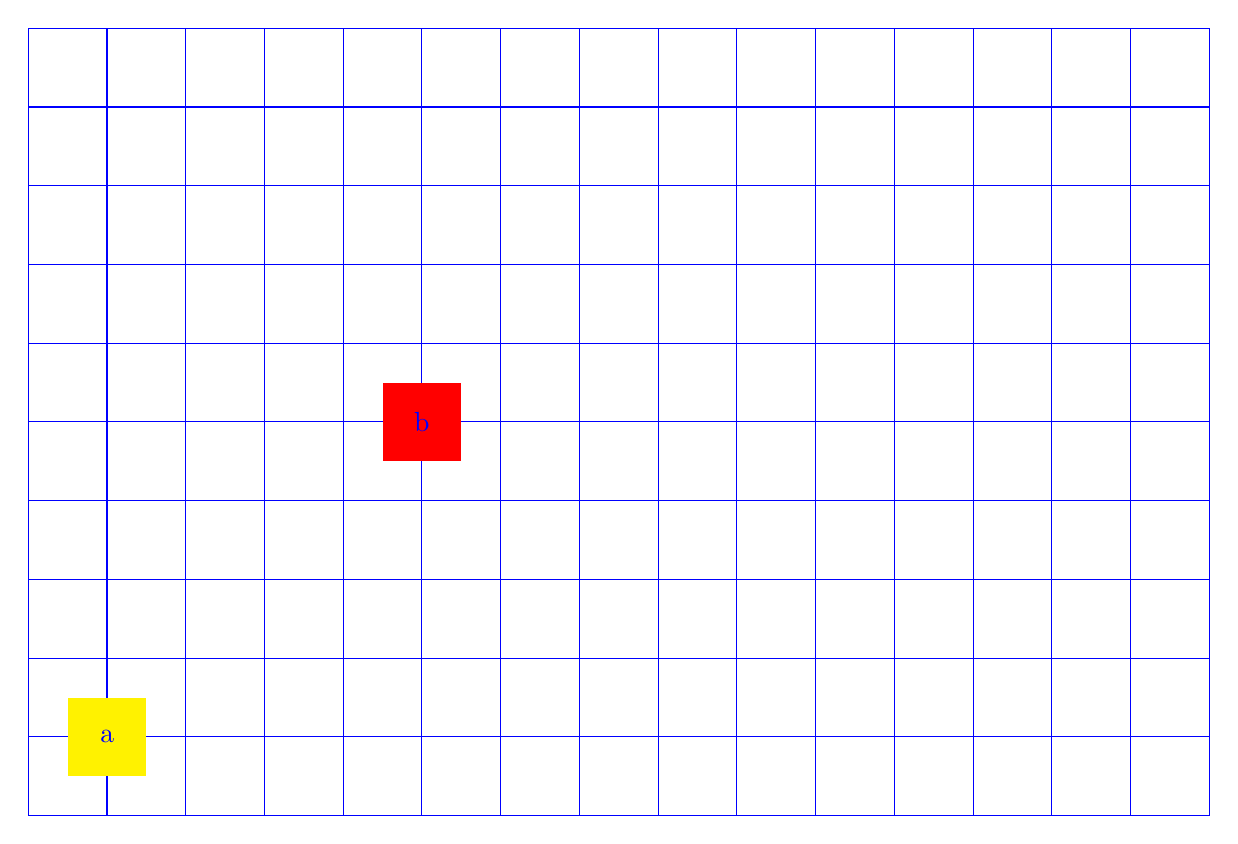
\begin{tikzpicture}[
punkt/.style={rectangle, minimum size = 1cm, blue, fill=yellow},
punktr/.style={punkt, fill=red},
]
\draw[help lines,blue,thin] (0,0) grid (15,10);

\node[punkt] (A) at (1,1){a};

\node[punktr] (B) at (5,5){b};

\end{tikzpicture}
\end{center}

\blindtext

% https://tex.stackexchange.com/questions/61805/tikz-using-loop-to-draw-grid-of-nodes
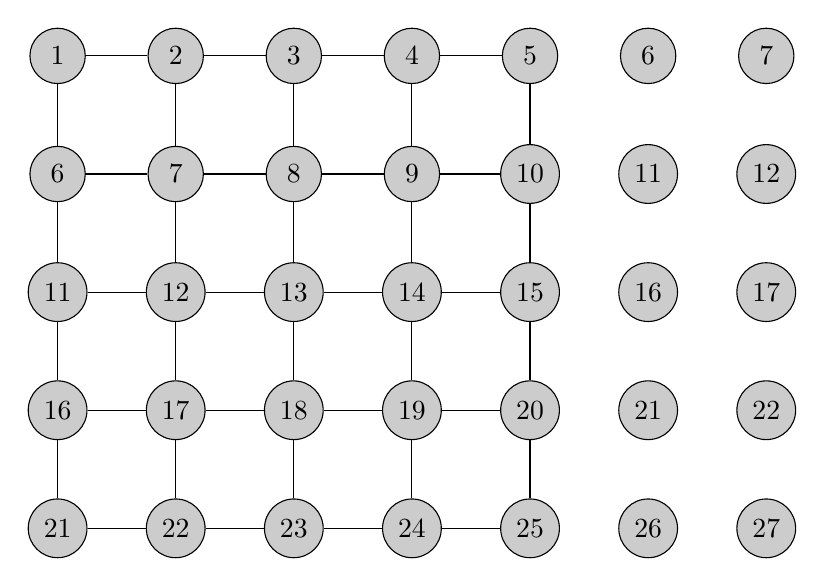
\begin{tikzpicture}[darkstyle/.style={circle,draw,fill=gray!40,minimum size=20}]
  \foreach \x in {0,...,6}
    \foreach \y in {0,...,4} 
       {\pgfmathtruncatemacro{\label}{\x - 5 *  \y +21}
       \node [darkstyle]  (\x\y) at (1.5*\x,1.5*\y) {\label};} 

  \foreach \x in {0,...,4}
    \foreach \y [count=\yi] in {0,...,3}  
      \draw (\x\y)--(\x\yi) (\y\x)--(\yi\x) ;

\end{tikzpicture}


\end{document}